\documentclass[a4paper,landscape]{article}
\usepackage[margin=0.8cm]{geometry}
\usepackage{tikz}
\usepackage{tikzfill}

\newcommand\wallHeight{2.5in}
\newcommand\coverHeight{0.5in}
\newcommand\buildingHeight{3in} % must be wallHeight + coverHeight
\newcommand\buildingWidth{7in}
\newcommand\buildingDepth{3.0in}

\newcommand\innerEps{0.5mm}
\newcommand\norm{1}
\newcommand\flip{-1}
\newcommand\flapWidth{0.8cm}
\newcommand\vflap[4]
{
\draw (#1, #2)
  -- ++(#4 * \flapWidth, -\flapWidth)
  -- ++(0, -#3 + 2 * \flapWidth)
  -- ++(#4 * -\flapWidth, -\flapWidth)
  -- cycle
  ;
}

\begin{document}
\pagestyle{empty}

\begin{tikzpicture}
  [ remember picture
  , overlay
  , line width=0.02cm
  ]

\begin{scope}[yshift=-\coverHeight]
\vflap{0}{0}{\buildingHeight}{\flip}
%\path[draw,fill tile image*={width=2.7in}{/home/mkl/sandbox/tabletop/terrain/textures/concrete/Concrete041B_1K-JPG_Color.jpg}] (0,0)
\path[draw,fill tile image*={width=2.7in}{/home/mkl/sandbox/tabletop/terrain/textures/concrete/PaintedPlaster010_1K-JPG_Color.jpg}] (0,0)

  rectangle ++(\buildingWidth,-\buildingHeight)
  rectangle ++(\buildingDepth,\buildingHeight)
  ;
\draw (0,0)
  rectangle ++(\buildingWidth, \coverHeight * 1.5)
  rectangle ++(\buildingDepth, -\coverHeight * 1.5)
  ;
\end{scope}

\begin{scope}[yshift=-4.5in]
\vflap{0}{0}{\buildingHeight}{\flip}
\draw (0,0)
  rectangle ++(\buildingWidth,-\buildingHeight)
  rectangle ++(\buildingDepth,\buildingHeight)
  ;
\draw (0,0)
  rectangle ++(\buildingWidth, \coverHeight * 1.5)
  rectangle ++(\buildingDepth, -\coverHeight * 1.5)
  ;
\end{scope}

\end{tikzpicture}




\newpage

\begin{tikzpicture}
  [ remember picture
  , overlay
  , line width=0.02cm
  ]


\begin{scope}[yshift=0cm]
%\path[draw,fill tile image*={height=3in}{/home/mkl/sandbox/tabletop/terrain/textures/solar-panel/SolarPanel003_1K-JPG_Color.jpg}] (0,0)
\path[draw] (0,0)
  rectangle ++(\wallHeight - \innerEps,-\buildingWidth + \innerEps)
  rectangle ++(\buildingDepth - \innerEps,\buildingWidth - \innerEps)
  rectangle ++(\wallHeight - \innerEps,-\buildingWidth + \innerEps)
  rectangle ++(\buildingDepth - \innerEps,\buildingWidth - \innerEps)
  ;
\vflap{0}{0}{\buildingWidth + \innerEps}{\flip}
\end{scope}

%\begin{scope}[xshift=12cm]
%\path[draw,fill tile image*={height=3in}{/home/mkl/sandbox/tabletop/terrain/textures/solar-panel/SolarPanel003_1K-JPG_Color.jpg}] (0,0)
  %rectangle ++(\wallHeight - \innerEps,-\buildingWidth + \innerEps)
  %rectangle ++(\buildingDepth - \innerEps,\buildingWidth - \innerEps)
  %;
%\vflap{0}{0}{\buildingWidth + \innerEps}{\flip}
%\end{scope}

%\begin{scope}[yshift=-0.5cm, xshift=17cm]
%\draw (0,0)
  %rectangle ++(\wallHeight - 2*\innerEps,-\buildingDepth + 2*\innerEps)
  %rectangle ++(-\wallHeight + 2*\innerEps,-\buildingWidth/2)
  %;
  %\begin{scope}[rotate=-90, yshift=\wallHeight - 2*\innerEps]
  %\vflap{0}{0}{\wallHeight + 2*\innerEps}{\flip}
  %\end{scope}
%\end{scope}

\end{tikzpicture}

\end{document}
